Liam Sharp$^1$, Grace Brannigan$^{1,2}$
Center for Computational and Integrative Biology, Rutgers University-Camden$^1$, 
Department of Physics, Rutgers University-Camden$^1$\\

\section{Abstract}
In model membranes \nachr~is functionally dependent on cholesterol and are modulated by anionic lipids. We showed previously that 1) \nachr~preferentially interacts with long acyl-chained and highly unsaturated polyunsaturated fatty acids (PUFAs) over shorter chained and less saturated PUFAs. 2) \plgic~inter-subunit and M4 have lipid specificity for raft forming lipids and PUFAs, respectively, with anionic lipids favoring sites with more cationic amino acids.  \nachr~boundary lipids in a native neuronal membrane are unknown. Using coarse grained molecular dynamics we simulate \nachr~embedded in a neuronal phospholipid membrane and analyze boundary lipids distribution and using a new approach for calculating binding affinities ($\Delta G$) predict \nachr~neuronal boundary lipid distributions. Cholesterol and neutral n-3 PUFAs had the strongest occupancy affinities of lipids simulated but had the strongest affinities for inter-subunit and M4 sites respectively. Anionic lipids were energetically unfavorable at the TMD in the outer leaflet but had the strongest affinities for inner M4 sites independent of acyl-chain or head group size. 

\section{Introduction}
\label{Intro}

The nicotinic acetylcholine receptor (\nachr)~is a well studied excitatory pentameric ligand gated ion channel (\plgic s). \nachr s~ are found at high density in post-synaptic membranes and the neuromuscular junction in mammals, and the electric organ in \textit{Torpedo} electric rays. \nachr~is activated by binding nicotine or acetylcholine in specific binding pockets in the extra-cellular domain (ECD) \cite{Dacosta2013,Guros2020}. When \nachr s are activated en-mass they stimulate an action potential. \nachr s~play a critical role in both cognition and memory\cite{Henault2015} and neuromuscular function \cite{Mukhtasimova2016,Kalamida2007}. \nachr~ and the greater \plgic~superfamily, play various roles in neurological diseases related to inflammation \cite{Taly2009,Cornelison2016,Patel2017,Yocum2017,Egea2015},  addiction \cite{Cornelison2016}, chronic pain \cite{Xiong2012}, Alzheimer's Disease \cite{Walstab2010,Picciotto_Neuroprotection_2008,MartinRuiz_4_1999,Kalamida2007},spinal muscular atrophy \cite{Arnold_Reduced_2004}, schizophrenia \cite{Haydar2010,Kalamida2007} and neurological autoimmune diseases \cite{Lennon_Immunization_2003, Kumari2008}.
%Egea2015

\nachr s~are highly sensitive to their local lipid environment. \nachr~is inactive in model phosphatidylcholine (PC) only membranes but can conduct a current with the addition of cholesterol \cite{Baenziger2017}, though too much or too little cholesterol can result in a loss of function \cite{M.CriadoH.Eibl1982}.  Previous studies using model membranes suggest cholesterol and anionic lipids \cite{Dalziel1980,Ellena1983,M.CriadoH.Eibl1982,Fong1986,Fong1987,Jones1988,Sunshine1994,DaCosta2009b} are required for \nachr~ function.  Functional studies using \xo~ \cite{Zhou2003,Gamba2005,Chen2015,Kouvatsos2016,Nys2016,Polovinkin2018,Moffett2019,Kumar2020} require lipid additives such as asolectin\cite{M.CriadoH.Eibl1982,Zhou2003,Gamba2005,Chen2015,Kouvatsos2016,Nys2016,Polovinkin2018,Moffett2019,Kumar2020} or synaptic membranes \cite{Conti2013} to return native ion flux to \nachr. It is unclear what specific lipid (or lipids) in \nachr's boundary lipid composition are essential to function in model membranes or its native neuronal membranes.%Why using addition membranes to restore function rather than cholesterol or anionic lipids is unclear \liam{not quite}. 

Mammalian neuronal membranes \cite{Isolated1969, Taguchi2010, Breckenridge1973,Ingolfsson2017b} have unique compositions compared to other mammalian membranes\cite{McEvoy2000,Kim2001,VanMeer2010,Lorent2020,Ingolfsson2014}. Neuronal membranes are more similar to \textit{Torpedo} electric ray's electric organ \cite{Barrantes1989a,Quesada2016} than the average mammalian membrane\cite{Ingolfsson2014}. Neuronal membrane \cite{Isolated1969, Taguchi2010, Breckenridge1973,Ingolfsson2017b} composition consists of several essential PUFAs, more specifically the $n-6$ PUFA arachidonic acid (AA), and the $n-3$ PUFAs docosahexaenoic acid (DHA) and eicosapentaenoic acid (EPA). These three PUFA's comprise a sizable fraction of neuronal phospholipids, and are involved in secondary signaling \cite{McNamara2008,Hamazaki2015} and neuronal development \cite{Maekawa2017}. PUFAs are linked to several of neurological diseases and disorders that overlap \nachr~related diseases. PUFAs play a roll in major depressive and bipolar disorder \cite{Adibhatla2007,McNamara2008,Schneider2017,Koga2019,Hamazaki2015}, schizophrenia \cite{Peet2003,Bushe2005,Berger2006,Schneider2017,Maekawa2017,Hamazaki2015}, and Alzheimer's Disease \cite{Conquer2000,DiPaolo2011,Bennett2013,Adibhatla2007,Yadav2014,Escriba2017}. %Unfortunately, the composition and \liam{microscopic properties} affect on embedded \plgic s is poorly understood.

It is experimentally challenging to capture the boundary lipid composition of \plgic~because lipids are small and fluid molecules. Functional experiments demonstrated anionic lipids and cholesterol as lipid modulators for \plgic's function  \cite{Ellena1983,Fong1986,Fong1987,Jones1988,Sunshine1994,DaCosta2009b}, but \plgic s are functional dependent on boundary cholesterol \cite{Dalziel1980,Addona1998,M.CriadoH.Eibl1982}. However, functional experiments require additional mutational studies or structural biology to determine where and which lipids bind. Structural biology has found potential cholesterol sites at subunit interfaces \cite{Laverty2017, Budelier2019}, specific phospholipid sites in the inter-subunit site \cite{Henault2019,Basak2017} and inter-subunit sites \cite{Kim2020}, and anionic lipids binding to inner inter-subunit sites \cite{Tong2019}. Fluid structures are difficult to resolve leaving lipids in, potentially, energetically unfavorable conformations, and structure replication cannot provide an average geometry for bound lipids.

Molecular dynamics (MD) simulations are a practical tool as MD specializes in molecular sized structures, fluids, and predicting structural significance of bound lipids. MD simulation has identified cholesterol \cite{Brannigan2008} interaction at inter-subunit sites and PUFAs at M4 sites\cite{Woods2019}, as well as anionic lipids binding at inner inter-subunit sites \cite{Tong2019}. 

With the growing use of coarse-grained molecular dynamics (CGMD) simulations, complex quasi-realistic membranes are becoming more practical. Ing{\'o}lfsson et al 2014 simulated and analyzed an ``average mammalian'' membrane containing 63 lipids species. In 2017, Ing{\'o}lfsson compared a coarse-grained neuronal membrane\cite{Ingolfsson2017b} to the average mammalian membrane. Accessible and simulatable realistic membranes are being expanded on, comparing the difference between model and quasi-realistic membranes and their protein interactions \cite{Marrink2019,Wilson2020,Ingolfsson2020,Carpenter2018,Lorent2019}. No such CGMD simulations using qausi-realistic membranes have been used with \plgic s.

Work by Sharp\cite{Sharp2019}, Woods\cite{Woods2019}, and Tong\cite{Tong2019} predict lipid distributions around \plgic s using model membranes. Based on our previous work \cite{Sharp2019, Woods2019, Tong2019}, we hypothesize a series of lipid occupancy sites for \nachr~based on acyl-chain saturation and head group charge, see Figure \ref{fig:trj}a. We predict PUFAs will occupy regions around the M4 alpha-helices, and raft forming lipids will occupy inter-subunit sites. Neutral lipids are predicted to occupy any site in the outer leaflet and inner leaflet inter-subunit sites, but anionic lipids will predominately occupy only the inner leaflet M4 sites, where there is a higher number of cationic amino acids.

The previous model membranes are significantly simplified compared to realistic membranes, i.e. 2-3 lipid species versus 10 or more. While model membranes are useful in predicting how lipid species may occupy sites, they have critical limitations. Model membranes do not consider how multiple lipids of similar acyl-chain saturation compete to bind to a \plgic~(i.e. n-3 PUFA EPA compared to DHA, or n-3 PUFA DHA and n-6 PUFA ALA). Nor do model membranes consider how various like-charged lipid head groups interact at the boundary region (i.e. which binds more PC or phosphoethanolamine (PE), phosphoserine (PS) or phosphoinositol (PI)). Determining \nachr's boundary lipid composition in native membranes is critical to understanding the receptor's function, or what lipid additives are required to prevent a lack of function.

For this work, we embed the neuromuscular \nachr\cite{Unwin2005} in a coarse-grained neuronal membrane \cite{Ingolfsson2017b}. To test this hypothesis we use polar enrichment density plots and occupancy affinity by free energy calculations. We find our hypothesis, based on model membranes, does not hold. Neutral lipids are more favorable in the outer leaflet, but n-3 PUFAs and cholesterol tend to occupy \nachr~sites indiscriminately. In the inner leaflet, neutral n-3 PUFAs and cholesterol tend to compete with anionic n-3 PUFAs and cholesterol tends to occupy inter-subunit sites, but anionic lipids occupy M4 regardless of acyl-chain saturation. 

\section{Methods}
\label{lab}

\subsection{Simulation Composition}
All simulations used the coarse-grained MARTINI 2.2\cite{DeJong2012} topology and forcefield.
\nachr~ coordinates were based on a cryo-EM structure of the $\alpha{\beta}\gamma\delta$ muscle-type receptor in native torpedo membrane (PDB 2BG9\cite{Unwin2005}). This is a medium resolution structure (4\AA) and was further coarse-grained using the martinize.py script; medium resolution is sufficient for use in coarse-grained simulation, and the native lipid environment of the proteins used to construct 2BG9 is critical for the present study. The secondary, tertiary and quaternary structure in 2BG9 was preserved via soft backbone restraints during simulation as described below, so any inaccuracies in local residue-residue interactions would not cause instability in the global conformation.  

\nachr~was embedded in a coarse-grained neuronal membrane based on Ing{\'o}lfsson et al 2017. The neuronal membrane from described by Ing{\'o}lfsson contains phospholipids, sterols, diacylglycerol, and ceramide. Membranes presented in this paper only consider phospholipids and cholesterol, for a total of 36 unique lipid species, see Table \ref{tab:rats}.

Coarse-grained membranes were built using the MARTINI script insane.py \cite{Wassenaar2015}, which was also used to embed the coarse-grained \nachr~within the membrane. The insane.py script randomly places lipids throughout the inter- and extra-cellular leaflets, and each simulation presented in this manuscript was built separately. Head-group and  acyl-chain compositions were dictated by Ingolfsson 2017 \cite{Ingolfsson2017b}. All simulation box sizes were $40x40x35$ nm$^3$ with  $\sim 4,500-5,000$ lipids and total $\sim450,000$ beads.

\subsection{Simulations}

Molecular dynamics simulations run using the MARTINI 2.2\cite{DeJong2012} forcefield and GROMACS\cite{Berendsen1995,Abraham2015}  2019.2 . All systems used van der Waals (vdW) and Electrostatics with reaction-field and a dielectric constant of $\epsilon_r$=15 and electrostatic cutoff length at 1.1 nm. Energy minimization was performed for 1000000 steps, but energy minimization tended to concluded after $\sim 5000-10000$ steps.

Volume and pressure equilibrations were run with isothermal-isochoric (NVT) and isothermal-isobaric (NPT) ensembles respectively. NVT and NPT simulations used a time step of 15 fs and run for 0.3 ns using Berendsen thermostat held at a temperature of 323 K, and Berendsen pressure coupling with compressibility set to 3$\times$10$^{-5}$ bar$^{-1}$ and a pressure coupling constant set to 3.0 ps  for the NPT ensemble. 

Molecular dynamics simulation were run using a time step of 20 fs for 5 $\mu$s for 10 replicas. Simulations were conducted in the NPT ensemble, by using the V-Rescale thermostat set to 323 K with temperature and a coupling constant set to 1 ps. Semi-isotropic pressure coupling was set to Parrinello-Rahman with compressibility at 3$\times$10$^{-5}$ bar$^{-1}$ and pressure coupling constant set to 3.0 ps. 

Secondary structures restraints consistent with MARTINI recommendations were constructed by the martinize.py \cite{DeJong2012} script and imposed by GROMACS \cite{Berendsen1995,Abraham2015}. \nachr~conformation was preserved by harmonic bonds between backbone beads separated by less than 0.5 nm and calculated using the ElNeDyn algorithm \cite{Periole2009} associated with MARTINI \cite{DeJong2012} with a coefficient of 900 kJ$\cdot$mol$^{-1}$.

\subsection{The Analysis}

Two-dimensional density distribution of the beads within a given lipid species $l$ around the protein was calculated on a polar grid:
  \begin{equation}
      \rho_{B}(r_i,\theta_j)= \frac{\left\langle n_{B}(r_i,\theta_j) \right\rangle}{r_i \Delta{r}\Delta{\theta}} \\        
    \label{eq:R}
  \end{equation}
  where  $r_i = i \Delta{r}$ is the projected distance of the bin center from the protein center, $\theta_j = j \Delta{\theta}$ is the polar angle associated with bin j,  $\Delta{r}$= 10\AA~ and  $\Delta{\theta} = \frac{\pi}{15}$ radians are the bin widths in the radial and angular direction respectively, and $\left\langle n_{B}(r_i,\theta_j) \right\rangle$ is the time-averaged number of beads of lipid species $B$ found within the bin centered around radius $r_{i}$ and polar angle $\theta_{j}$.  In order to determine enrichment or depletion, the normalized density $ \tilde{\rho}_{B}(r_i,\theta_j)$ is calculated by dividing by the approximate expected density of beads of lipid type B in a random mixture, $x_{B}s_{B}~N_{L}/\langle L^{2}\rangle$, where $s_{B}$ is the number of beads in one lipid of species B, $N_{L}$ is the total number of lipids in the system, and $\langle L^{2}\rangle$ is the average projected box area:
  \begin{equation}
  \tilde{\rho}_{B}(r_i,\theta_j)=\frac{ \rho_{B}(r_i,\theta_j)}{x_{B}s_{B}~N_{L}/\langle L^{2}\rangle} \\        
    \label{eq:Rt}
  \end{equation}
where the expected density is derived at the first frame of the simulation.
 
 
This expression is approximate because it does not correct for the protein footprint or any undulation-induced deviations of the membrane area.  The associated corrections are small compared to the membrane area and would shift the expected density for all species equally, without affecting the comparisons we perform here. 

We defined 20 occupancy sites around \nachr's TMD: 5 inter-subunit sites and 5 M4 sites in both outer and inner leaflets. Occupancy sites are defined using polar density analysis, see Figure \ref{fig:PBT}b for site deffinitions. Site occupation does not follow the standard ``a ligand is occupied or unoccupied'' model, instead we consider partial occupation. Partial occupancy ranges from fully occupied, partially occupied, or unoccupied. A site is fully occupied if a single lipid species (A) is the only lipid species occupying a site. Like the small molecule displaced by water, a portion of lipid A may be partially or fully displaced by a second lipid (B).  

Affinity is defined as the change in the Gibbs' free energy ($\Delta G$). $\Delta G$ is calculated using two probability distributions, $P_{occ}$ and $P_{bulk}$, see Figure \ref{fig:PBT} a. Both distributions are calculated from the time averaged number of lipid beads within the area of an occupancy site ($P_{occ}$) or an identical area in the bulk membrane ($P_{bulk}$).  
To calculate the affinity, we define $P_{<}$ and $P_{>}$
\begin{subequations}
    \begin{align}
    %P_{<} \equiv \big\{\sum P_{occ} \leq \big< P_{bulk} \big> \big\} \label{eq:Pl} \\
    %P_{>} \equiv \big\{\sum P_{occ} > \big< P_{bulk} \big> \big\} \label{eq:Pg}
    P_{<} \equiv \sum P_{occ} \leq \big< P_{bulk} \big> \label{eq:Pl} \\
    P_{>} \equiv \sum P_{occ} > \big< P_{bulk} \big> \label{eq:Pg}
    \end{align}
\end{subequations}

Using the mean value of $P_{bulk}$ ($ \big< P_{bulk} \big> $) as a reference, the sum of $P_{occ}$ less than or equal to   $\big< P_{bulk} \big> $ is defined as $P_{<}$. The sum of  $P_{occ}$ greater than  $\big< P_{bulk} \big> $ is defined as $P_{>}$. The affinity is then defined as the overlap between $P_{<}$ and $P_{>}$.

\begin{equation}
\Delta G = -RT\ln\frac{P_{>}}{P_{<}}
\label{eq:dG}
\end{equation}

Where RT is the gas constant R and the temperature of the simulation. The stronger the affinity the smaller the numeric value.

The area of an occupancy site ($A_s$) is the sum of the area accessible to the lipids ($A_{acc_s}$) and the area restricted to the lipids by the protein ($A_{rest_s}$): $A_s = A_{acc_s} + A_{rest_s}$.  $A_s$ values are calculated on a polar plane, see Figure \ref{fig:PBT} b. $A_s$ for inter-subunit and M4 sites are determined by non-overlapping angular and radial bin densities. Inter-subunit sites are determined by the angular component of bins between two adjacent subunits' M1 and M3 alpha-helices and the radial component is $10<r\leq32$ $\AA $.  M4 sites are determined by the angular component given by the set of bins within one subunit using M1 and M3 alpha-helices and the radial component is $10<r\leq44$ $\AA$. The area for each site is calculated by:

\begin{equation}
    A_s = \frac{\left\langle n_s(r,\theta) \right\rangle}{\rho_s(r,\theta)}
\label{eq:A}
\end{equation}

Where $\left\langle n_s(r,\theta) \right\rangle$ is the associated time averaged number of beads within a polar bin and $\rho_s$ is the time averaged numeric bin density, see eq \ref{eq:R}. Only values of $\left\langle n_s(r,\theta) \right\rangle$ and  $\rho_s$ within the range of angular and radial bins described above are used. For the affinity calculation described above the bin radial and angular widths are $\Delta r=$  4$\AA$ and $\Delta \theta=$ $\frac{\pi}{25}$. Using the values calculated for $A_s$, we calculate $A_{acc}$ to determine accurate bulk areas for $P_{bulk}$.

\begin{equation}
	A_{acc_s} \equiv \frac{\left\langle n_{occ_s} \right\rangle A_s }{\left\langle n_s \right\rangle} \label{eq:aac}\\
\end{equation}

$\left\langle n_{occ_s}\right\rangle$ and $\left\langle n_s  \right\rangle$ are the average number of lipid beads for a specific occupancy site and the average number of lipid beads in the bulk membrane within a given area $A_s$. The values for $A_{acc_s}$ are then used to calculate $P_{bulk}$, see Figure \ref{fig:PBT} a.

\begin{figure}[!h]
	\center
	%\includegraphics[width=\linewidth]{PartialBIndingToy.pdf}
	\includegraphics[width=4in]{Figures/PartialBIndingToy.pdf}

	\caption[ Model distribution used for calculating affinity and occupancy site definitions.] {Model distribution used for calculating affinity and occupancy site definitions. a)  Toy $P_{occ}$ and $P_{unocc}$ distributions in red and blue curves respectively. Black line shows mean value of $P_{unocc}$. $P_<$ (pink) is the sum of  $P_{occ}$ less than and equal to  $P_{unocc}$'s mean value. $P_>$ (light blue) is the sum of  $P_{occ}$ greater than $P_{unocc}$'s mean value. b) Binding site area's. Black and white represent areas for inter-subunit and M4 occupancy sites, respectively. Grey show sites not considered for occupancy areas.}
	\label{fig:PBT}
\end{figure}



\section{Results and Discussion}
\label{res}

\begin{figure*}[!h]
	\center
	\includegraphics[width=4in]{./Figures/acyl_heatmap.pdf}
	%\includegraphics[width=\linewidth]{acyl_heatmap.pdf}
	%55mm]{acyl_heatmap.pdf}
	\caption[Model binding areas and acyl-chain density enrichment or depletion around a central singular \nachr.] { Density enrichment is calculated using eq \ref{eq:Rt} for both outer and inner leaflet columns, averaged over 10 replicas for 2.5 $\mu s$ each. The maximum radius from pore of \nachr~ is $60 \AA$. $\tilde{\rho}_{a}< 1$ describes acyl-chain depletion compared to a random bulk mixture, $\tilde{\rho}_{a}=0$ describes the expected mixture, and $\tilde{\rho}_{a}  > 1$ describes acyl-chain enrichment compared to a random mixture. a) Density enrichment based on acyl-chains, b) density enrichment based on head group charge.}
	\label{fig:acyl_map}
\end{figure*}

\subsection{Effect of Acyl-Chain on Neutral Lipid Affinities}

%\textit{SECTION 3.1:  EFFECT OF ACYL CHAIN ON NEUTRAL LIPID AFFINITIES a) Results block for figure 2.  b) Results block for figure 3 (neutral)  c) Results block for figure 4 (neutral). Results blocks in all three cases should be focused on role of unsaturation/chain flexibility.}

Results from Woods et al 2019 \cite{Woods2019} predict lipid occupancy sites for PUFAs and raft forming lipids at M4 and inter-subunit sites respectively. We hypothesize both neutral PUFAs and raft forming lipids will tend occupy M4 and inter-subunit sites in both leaflet. To test this hypothesis, we use radial enrichment densities (see eq \ref{eq:Rt}) and calculated affinities as $\Delta G$ values, described in methods and equations \ref{eq:A}-\ref{eq:dG}.

\begin{figure*}[!h]
	\center
	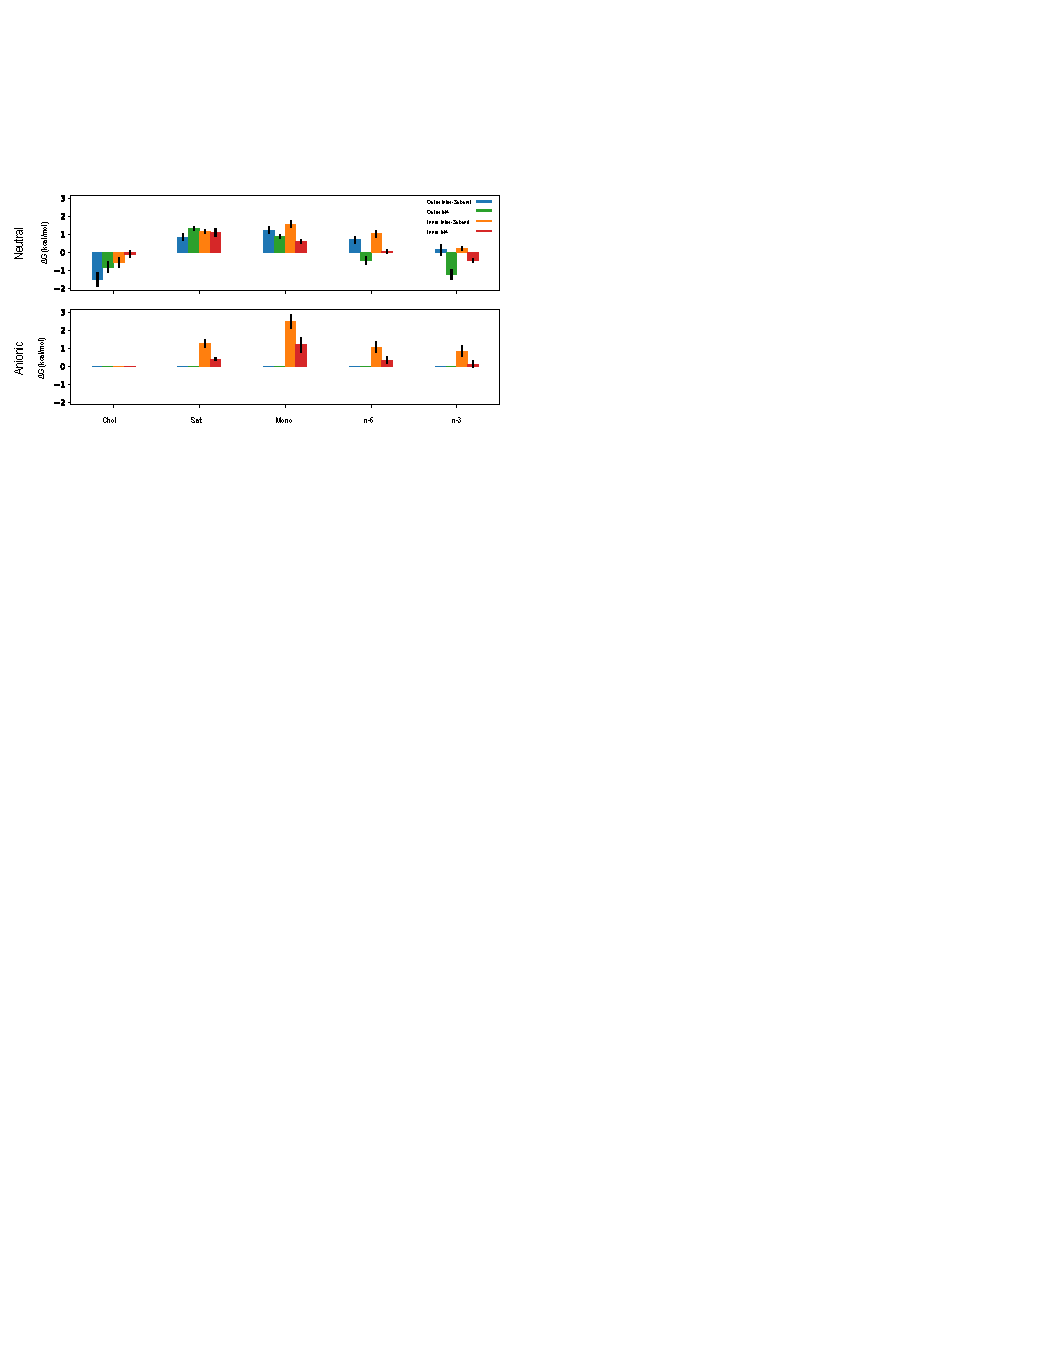
\includegraphics[width=\linewidth]{Figures/Protein_centric.pdf}
	\caption[Affinity calculation ranking for neutral and anionic lipid saturation species averaged over last half of 10 5$us$ replicas by charge.] {Affinity calculation ranking for neutral and anionic lipid saturation species averaged over last half of 10 5$us$ replicas by charge. Occupancy sites are averaged over each site type. Columns are lipid saturation, rows are charge, and colors represent a lipid occupancy site. The smaller the number the stronger the affinity.  Colors: Outer Inter-Subunit:blue, Outer M4:green, Inner Inter-Subunit:orange, Inner M4:red}
	\label{fig:proBar}
\end{figure*}

In order to compare the lipid distributions for the native system to our previous model system, we plotted enrichment densities for acyl-chains around the protein based on degree of saturation, and cholesterol, see Figure \ref{fig:acyl_map}a. Saturated and monounsaturated fatty acids have an approximately random distribution. Cholesterol, with the exception of specific annulus sites, is depleted in both leaflets. Both n-6 and n-3 PUFAs are symmetrically enriched around the M4 alpha-helixes, but have non-uniform enrichment around the inter-subunit regions in the outer leaflet. The PUFA area of enrichment decreases in the inner leaflet, where n-3 PUFAs show strong enrichment around the annulus of the protein but n-6 enrichment values are depleted to expected. These results diverge from what we saw in Woods et al\cite{Woods2019}. In our previous model membranes, we had well-defined five fold enrichment for n-3 PUFAs, in the native membranes, the boundaries become blurred. To determine concise lipid occupational information, 2D density are dimensionally reduced to calculate $\Delta G$ affinities for each site.

Using affinity calculations, eq \ref{eq:dG}, we compare inter-subunit and M4 site occupation affinities across neutral lipid acyl-chain saturations and cholesterol, where the smaller the value the stronger the affinity, see Figure \ref{fig:proBar}. Saturated and monounsaturated lipids generally have the weakest affinities for all sites.  Neutral PUFAs and cholesterol have the strongest affinities across all sites. n-3 PUFAs have affinity values approximately 0.2 kcal/mol for inter-subunit sites for both leaflets, $>$0.5 kcal/mol smaller than saturated lipid affinities. Unlike phospholipids, cholesterol has strong affinity values for all sites, but has stronger affinities for inter-subunit  than the M4 sites.

Figure \ref{fig:lipidBar} analyzes occupancy site affinity for acyl-species, and is sorted by charge and leaflet. Cholesterol has the strongest affinity of the neutral lipids at inter-subunit sites for both leaflets, but inner inter-subunit sites affinity is $\sim 50 \%$ weaker. Neutral phospholipids at inter-subunit affinity values change $<0.5$ kcal/mol between leaflets.  Inter-subunit and M4 have different affinities trends: n-3 $<$ n-6 $<$ saturated $<$ monounsaturated and  n-3 $<$ n-6 $<$ monounsaturated $<$ saturated respectively. 
 %At the M4 sites, n-3 PUFAs interact more favorably than other lipids 

%\subsubsection{Discussion}

The affinity results we observe reinforce what is shown in the 2D enrichment plots, Figure \ref{fig:acyl_map}, where n-3 PUFAs can occupy most regions of the TMD. We argue cholesterol's strong affinity for most sites have been averaged out in enrichment density plots but can be seen in Figure \ref{fig:lipidDist}, which provides lipid bead distributions.

Of the neutral lipids, n-3 PUFAs and cholesterol stand out. We predict the relative high affinity for n-3 PUFAs are a result of their flexibility. The n-3 PUFA, DHA, has several of unique membrane properties \cite{Stillwell2003a,Gawrisch2003}, and is observed to consistently interact with non-annular sites in and around \plgic s \cite{Sharp2019, Woods2019}. The inherent disorder in PUFAs and the strong affinity they have for M4 sites suggests PUFAs may minimize unfavorable membrane deformation\cite{Brannigan2005a,Brannigan2007,Hu2012a,Argudo2016,BuganzaTepole2017,Dan1993,Fournier2015} around \plgic's conical-star shape provided by M4. 

Cholesterol is rigid but the smallest of the lipids looked at, which potentially allows it to embed between alpha-helices. Brannigan et al 2008 \cite{Brannigan2008} hypothesized 3 non-annular cholesterol binding sites per subunit for \nachr. Sharp et al 2019 \cite{Sharp2019} observed cholesterol embedded in $\beta$ subunits of \nachr. It could be cholesterol's favorability for M4 is a result of its relative small size making it ideal for packing between alpha-helices.

For most sites monounsaturated lipids have the weakest affinities ($>.5$ kcal/mol). We hypothesize this is due to packing limitation from monounsaturated lipids single acyl-chain kink. Cholesterol and PUFAs are small or highly flexible and readily fit at various sites in \plgic's topology. Saturated lipids, lack double bonds and are more rigid than unsaturated lipids, may pack around inter-subunit site's ``flat'' topology. We argue the single acyl-chain kink found in monounsaturated lipids may prevent packing of itself around inter-subunit sites, and is not flexibility to compete with PUFA's occupying M4 sites. 

\begin{figure*}[!h]
	\center
	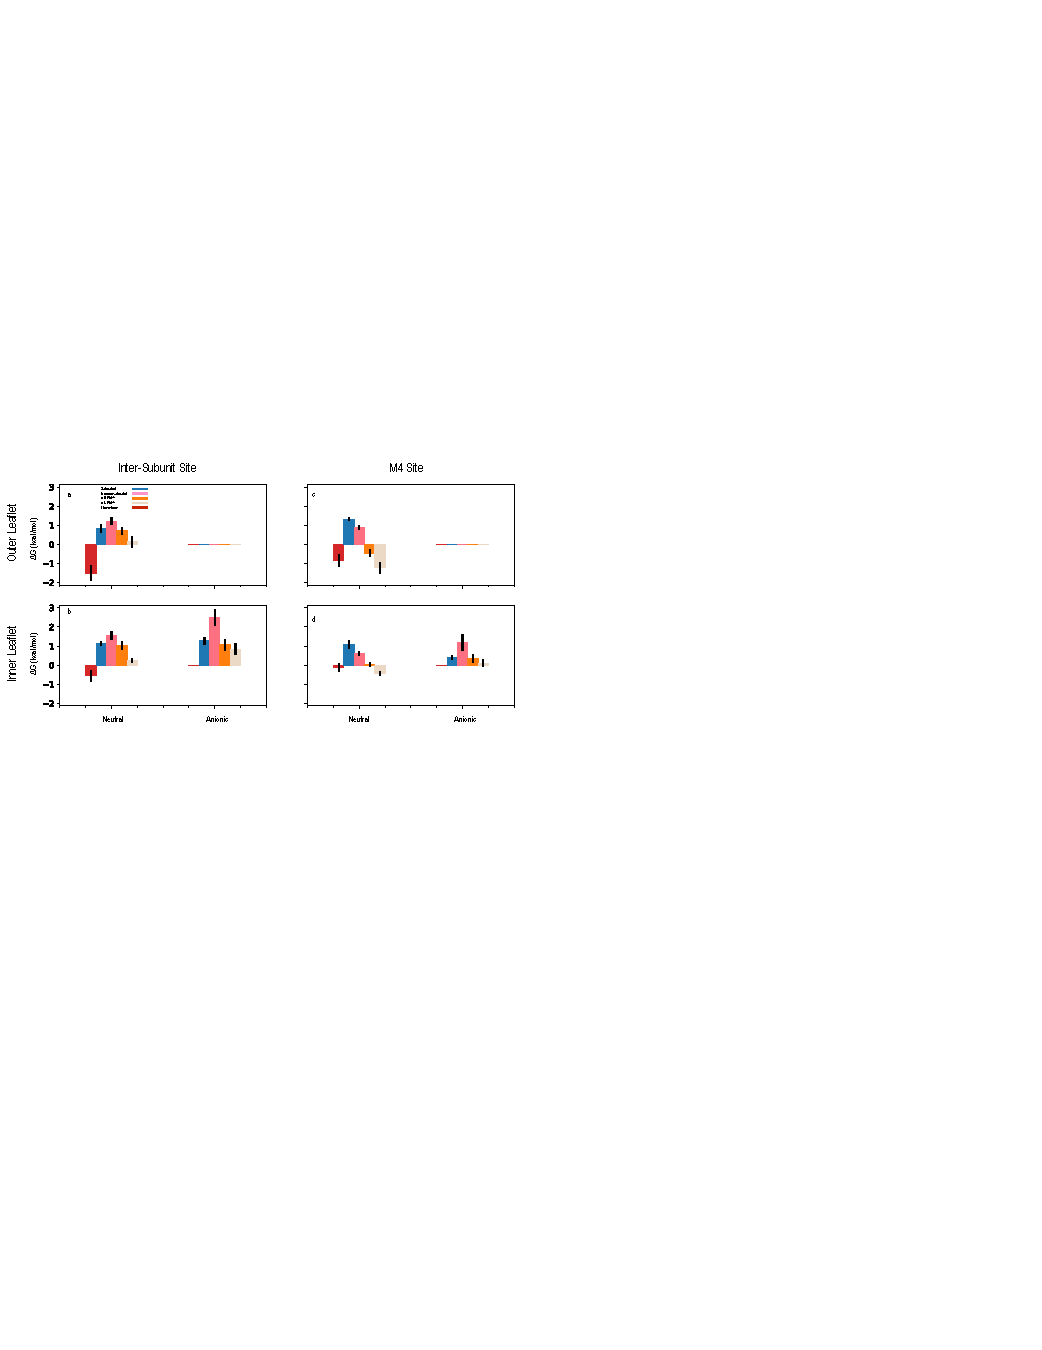
\includegraphics[width=\linewidth]{Figures/Lipid_centric.pdf}
	\caption[Affinity calculation ranking for neutral and anionic lipid saturation species averaged over last half of 10 replicas by occupancy site.] {Affinity calculation ranking for neutral and anionic lipid saturation species averaged over last half of 10 replicas by occupancy site. Occupancy sites are averaged from 20 sites. Row one is the outer leaflet and row two is the inner leaflet. Columns are charge, each subplot is a difference occupancy site. The smaller the number the stronger the affinity. Colors: Saturated:blue, Monounsaturated:green, n-6 PUFAs:orange, n-3 PUFAs:red, Cholesterol:purple}
	\label{fig:lipidBar}
\end{figure*}

\subsection{Effect of Head Group Charge on Affinity Depends on Leaflet and Binding Site}

Research by Tong et al 2019 \cite{Tong2019} showed anionic lipids favorably occupied around arginines in ELIC's inner inter-subunit site. We hypothesize \nachr's outer TMD and inner inter-subunit sites will have a strong affinity for neutral phospholipids and \nachr's inner M4 sites will have a strong affinity for anionic phospholipids because M4 has more cationic amino acids, see Figure \ref{fig:aaa}a. We test the proposed lipid distributions using both enrichment density analysis and affinity calculations.

We analyze the distribution for both neutral and anionic lipids using polar enrichment density plots, see Figure \ref{fig:acyl_map}b. Neutral lipids in the outer leaflet have weak enrichment around the M4 subunits and are approximately randomly distributed around the rest of the protein. Anionic lipids are not present in the outer leaflet at the start of simulations and change leaflets infrequently. Neutral lipids in the lower leaflet have an approximately random distribution. Anionic lipids are enriched at inner inter-subunit sites. However, anionic lipids are non-uniformly enriched around inner non-$\alpha$-subunit M3/M4 helices, see in Figure \ref{fig:acyl_map}b for $\alpha_{\gamma}, \gamma,\delta,$ and $\beta$. Non-$\alpha$ subunits have cationic amino acids closer to M4 alpha-helices, see Figure \ref{fig:aaa}a.

%We hypothesize the difference in our result is from the number and placement of charged amino acids in ELIC's (TMD PDB:3RQW\cite{Pan2012}) versus that of neuromuscular \nachr. We use VMD \cite{HUMP96} to visualize the difference between \nachr~and ELIC's inner \notsure{leaflet} TMD, . Both pLGICs have a number of cationic amino acids around their annulus. ELIC has more cationic amino acids embedded in the protein density than at the annulus. \notsure{Cationic amino acids found in the \nachr~structure tend to be more outward facing than cationic amino acids in the ELIC structure.} Non-$\alpha$ \nachr~ subunits have cationic amino acids closer to M4 alpha-helices. ELIC has cationic amino acids closer to the inter-subunit sites. Anionic amino acids are found at \nachr M4 alpha-helices, with the exception of the $\beta$ subunit. Anionic amino acids are found closer to the M1/M4 alpha-helices interfaces in ELIC, or embedded within the \liam{inner/non-annular/bulk of} protein.

Using affinity calculations derived from polar densities, eq \ref{eq:dG}, we analyze the affinities for neutral and anionic lipids in the outer leaflet for both sites, see Figure \ref{fig:lipidBar}. As in \textit{Effect of Acyl-Chain on Neutral Lipid Affinities}, the stronger the affinity the smaller the number. Anionic lipid have poor affinity for the TMD in the outer leaflet, $\geq 2.0$ kcal/mol. There is a noticeable neutral and anionic trend at inter-subunit sites: n-3 PUFAs $>$ n-6 PUFAs $>$ saturated $>$ monounsaturated.  %In the outer leaflet, \nachr~ has preferential binding with cholesterol, neutral PUFAs, and then monounsaturated or saturated, the later are dependent on site.  

\begin{figure}[!h]
	\center
	%\includegraphics[width=\linewidth]{Anonic_AA.pdf}
	\includegraphics[width=2in]{Figures/Anonic_AA.pdf}
	\caption[Charged amino acid representation in the TMD/ECD interface and ELIC anionic enrichment.] {Charged amino acid representation in the TMD/ECD interface and ELIC anionic lipid enrichment. a) Inner cellular view up of \nachr~(top) and ELIC (bottom). \nachr~ is color coded by subunit ($\alpha$:green, $\beta$: purple, $\delta$: grey, $\gamma$: cyan), ELIC is cyan. Cationic amino acids are colored in blue while anionic lipids are colored in red for both structures. b) Anionic polar density enrichment observed in ELIC, derived from \cite{Tong2019}. Grey circles represent center of mass of alpha-helices, red circles represent center of mass of alpha-helices with cationic amino acids. $\tilde{\rho}_{a}< 1$ describes acyl-chain depletion compared to a random bulk mixture, $\tilde{\rho}_{a}=0$ describes the expected mixture, and $\tilde{\rho}_{a}  > 1$ describes acyl-chain enrichment compared to a random mixture.}
	\label{fig:aaa}
\end{figure}

Occupancy affinities for neutral and charged lipids in inner inter-subunit sites are compared in Figure \ref{fig:lipidBar}. Saturated and n-6 PUFA affinity values for inner inter-subunit sites are similar independent of charge. Neutral n-3 PUFAs have a stronger affinity than anionic n-3 PUFAs, a difference of $\sim$0.5 kcal/mol. Neutral lipids in the inner leaflet have slightly weaker affinities than in the outer leaflet, difference $< 0.4$ kcal/mol. Anionic affinities are more favorable at inner inter-subunit sites than the outer leaflet, difference $\sim1.0$ kca/mol, excluding monounsaturated lipids. Similar to outer inter-subunit sites neutral and anionic lipids share a similar non-monotonic affinity trend.% have $\sim 1.0$ kcal/mol stronger affinity for the inter-subunit sites than in the outer leaflet.

We compare the relative affinities for neutral and anionic lipids in the inner M4 sites, see Figure \ref{fig:lipidBar}. Neutral and anionic lipids have different affinity trends for M4. Neutral lipid affinities are related to the acyl-chain flexibility while anionic lipids are non-monotonic. Neutral PUFAs and cholesterol have the strongest affinity values, $\leq 0$ kcal/mol.  Anionic lipids are generally $<0.6$ kcal/mol, excluding monounsaturated lipids, and have stronger affinities at M4 than at inter-subunit sites, independent of saturation. The average anionic affinity difference between inter-subunit and M4 sites is $\sim -1.0$ kcal/mol, see Figures \ref{fig:proBar} and \ref{fig:lipidBar} and Table \ref{tab:dGTab}. 

%\subsubsection{Discussion}
Binding sites show clear specificity for particular head group charge and acyl-chain saturation, suggesting \nachr~lipid occupancy to be driven in two steps, a ``coarse-sorting'' by head groups, and then ``fine-sorting'' by acyl-chains. In the outer leaflet anionic lipids are clearly unfavorable, this demonstrates coarse-sorting. A neutral lipid will occupy \nachr's boundary region but acyl chains dictate where specific lipids occupy \nachr, this demonstrates fine-sorting. It appears that fine-sorting does not occur for anionic lipids at inner M4, possibly due to the number of cationic amino acids at the M4 site. %diverge from this pattern at the inner M4 site which has the strongest affinity for anionic lipids independent of saturation. 

A potential mechanism for anionic lipid site occupation could be anionic lipids occupy M4 due to the number of positively charged amino acids until the site is saturated with anionic lipids, similar to Tong et al\cite{Tong2019}. The remainder anionic lipids do not all defuse back to the bulk membrane, they weakly interact with the inner inter-subunit site as a local anionic lipid pool for M4. 

\subsection{Effect of Head Group Details on Lipid Affinities}
%The NEW SECTION 3.3 : EFFECT OF HEADGROUP DETAILS ON LIPID AFFINITIES can instead be focused on the effect of specific headgroups

%Neutral lipids have a higher affinity in the outer leaflet. Neutral and anionic lipids show a level of competition at inner inter-subunit sites.  Anionic lipids have an acutely stronger affinity at inner M4 sites compared to neutral lipids. 

Neutral and anionic are bulk terms that categorize numerous lipid head-groups by charge. Frequently head group charge and size play a factor in direct protein-lipid interactions. Here we look at a few particular head groups species with the strongest affinities for occupying \nachr~by leaflet and site.

We show head group affinities in the outer leaflet site, see Table \ref{tab:dGOuterHG}.  Lipids with the small neutral head group PE have the highest affinity in both inter-subunit and M4 sites, -0.2$\pm$0.3 and -1.1$\pm$0.2 kcal/mol respectively and bulkier neutral PC and sphingolipids (SM) are weaker by $\sim > 0.5$ kcal/mol. Sharp et al 2019\cite{Sharp2019} and Tong et al 2019\cite{Tong2019} observed slightly more enrichment of PE than PC around pLGICs. In living cells PUFAs are frequently tethered to PE more than to PC or SM \cite{Isolated1969, Taguchi2010, Breckenridge1973,Ingolfsson2017b,Gamba2005,Lorent2020}. Anionic lipids are unfavorable with affinity values for PS and PI are both above 2 kcal/mol, and PIPS and PA above 3.5 kcal/mol.

Table \ref{tab:dGInnerHG} shows specific head group affinities in the lower leaflet. Anionic lipids have a stronger affinity in the inner leaflet compared to the outer leaflet, especially at the M4 sites. PE has the strongest affinity compared to anionic and other neutral lipids for both sites. Both PI and PS are $\sim 0.4 $ and $\sim 0.6$ kcal/mol weaker than PE (inter-subunit and M4 respectively), but PI and PS are $\sim 0.1$ and $\sim0.4$kcal/mol stronger than PC at inter-subunit and M4 sites respectively. Other anionic lipids, phosphatidic acid  (PA )and phosphoinositides (PIPS) have affinity values $>2.2$ and $>1.8$ kcal/mol for inter-subunit and M4 sites respectively.

%\subsubsection{Discussion}

It is unclear why PE is more favorable at this time. It may be due to the frequency which PE are attached to PUFAs or the size of the head group.  However, many of the the anionic lipid head groups are attached to PUFAs and if head group size were the leading factor, PS would be expected to have a greater occupancy affinity than PI lipids, as PS is smaller. It may be a product of head group to acyl-chain combination, \nachr~evolved to preferentially interact with specific head groups, or an artifact in the coarse grained model as PA is associated with \nachr~function in experimental model membranes \citep{Hamouda2006a,Cheng2007,Hung2011}. %The PE head group bead types are Qd and Qa, which are attracted to most of the other bead types. PS has P5 which is attractive to about half the bead types and repulsive to the other half. PI has coarse-grained ring of P5 and P1s, and Qa, all of which tend to be attractive to other beads. 

 \begin{figure*}
	\center
	\includegraphics[width=5in]{Figures/Trajectory.pdf}
	%\includegraphics[width=3in]{Trajectory.pdf}

	\caption[Trajectory of \nachr~boundary lipids in a native membrane.] {Trajectory \nachr~boundary lipids in a native membrane. Colors for all VMD images are: $\alpha$-subunits:green, $\gamma$-subunits cyan, $\delta$-subunits:grey, $\beta$-subunits:purple, saturated lipids: blue, monounsaturated lipids:orange, n-6 PUFAs:pink, n-3 PUFAs:beige, and cholesterol:red. a) Frames from neuronal membrane trajectory over 5 $\mu s$. \nachr is depicted using van der Waals beads and transparent quicksurf. Only lipid acyl chains are shown using van der Waals. Lipids are shown within 15 $\AA$ of \nachr. b) Inter-subunit and M4 sites and lipids with the strongest and weakest binding affinities. }
	\label{fig:trj}
\end{figure*}

\begin{table}
	\caption{Outer Leaflet $\Delta$G affinities for lipids based on head groups. Head groups are sorted by inter-subunit.}
    \centering
    \begin{tabular}{|l||c|c|}
    \hline
	{} &  Outer Inter Sites&  Outer M4 Sites\\
	{} & kcal/mol & kcal/mol\\
	\hline
	PE	&-0.2 $\pm$ 0.3& -1.1$\pm$0.2\\
	PC	& 0.8 $\pm$0.3 &  0.5$\pm$0.2\\
	SM	&1.9$\pm$0.3 &  1.7$\pm$0.1\\
	PS	&2.5$\pm$0.4 &  2.4$\pm$0.4\\
	PI	&2.8$\pm$0.5 &  2.6$\pm$0.4\\
	PIP3 &4.1$\pm$0.5 &  3.8$\pm$0.6 \\
	PIP1 &4.1 $\pm$0.5&  4.0$\pm$0.5\\
	PA &4.3 $\pm$0.4&  4.1$\pm$0.5\\
	PIP2 &4.6 $\pm$0.3&  4.5$\pm$0.4\\
	\hline
    \end{tabular}
    \label{tab:dGOuterHG}
\end{table}

\begin{table}
	\caption{Inner Leaflet $\Delta$G affinities for lipids based on head groups. Head groups are sorted by inter-subunit.}
    \centering
    \begin{tabular}{|l||c|c|}
    \hline
	{} &  Inner Inter Sites&  Inner M4 Sites\\
	{} & kcal/mol & kcal/mol\\
	\hline
	PE& 0.3$\pm$0.2& -0.1$\pm$0.1\\
	PI&0.9$\pm$0.3 &  0.2$\pm$0.1\\
	PS&1.0 $\pm$0.2	&  0.4$\pm$0.1\\
	PC&1.2 $\pm$0.2	&  0.7$\pm$0.1\\\
	SM&2.2 $\pm$0.4	&  1.4 $\pm$0.1\\
	PIP3	&2.6$\pm$0.4	 &  1.8 $\pm$0.4\\
	PIP2	&2.8 $\pm$0.2	&  2.1$\pm$0.4\\
	PIP1	&2.4 $\pm$0.3	&  2.1$\pm$0.4\\
	PA	&3.0 $\pm$0.3	&  2.2$\pm$0.4\\
	\hline
    \end{tabular}
    \label{tab:dGInnerHG}
\end{table}

\section{Conclusions}

\label{con}

 
We used a neuronal lipid compositions modified from\cite{Ingolfsson2017b} to analyze \nachr~within a neuronal membrane. We defined lipid-protein occupancy from polar density analysis and used Sharp\cite{Sharp2019}, Woods\cite{Woods2019}, and Tong\cite{Tong2019} to hypothesize specific lipid occupancy for each site. We hypothesized that PUFAs and raft forming lipids would occupy the M4 and inter-subunit sites respectively, while anionic lipids would occupy inner M4 site of \nachr. Our results show lipid distributions among occupancy sites differ from our hypothesis.

Of the phospholipids analyzed, n-3 PUFAs have the strongest affinities across all sites, with affinities values of $\sim<0$ kcal/mol for M4 sites and $\sim<$.5 kcal/mol for inter-subunit sites. Similar to n-3 PUFAs, cholesterol occupies sites nearly indiscriminately, though for each leaflet cholesterol has the strongest affinity at inter-subunit site. Cholesterol's affinity for the M4, compared to inter-subunit sites, is reduced by about $50\%$ and $80\%$ for the outer and inner leaflets respectively. However, unlike the phospholipids, cholesterol's affinity for each site is consistently $<0$ kcal/mol. 

Neutral lipids have a stronger affinity for the outer leaflet compared to anionic lipids. Neutral lipids found at the inner inter-subunit sites have slightly weaker affinities compared to the same lipids in the outer inter-subunit site. Anionic lipids have stronger affinity for inner M4 than inner inter-subunit sites. Inner anionic saturated, n-6 and n-3 PUFAs have significantly greater affinities than outer anionic lipids of the same saturation types. Monounsaturated lipids affinity values do not change much between leaflets ($\sim 0.5$ kcal/mol). We associate anionic lipids have stronger affinity for M4 in \nachr~compared to ELIC due to cationic amino acid distribution, see Figure \ref{fig:aaa}a. \nachr~ has cationic amino acids at both inter-subunit and M4 sites.

For both outer and inner leaflets neutral lipids with smaller head groups PE have stronger affinity than the larger PC or SM. Anionic lipids in the lower leaflet have some what of an inverse relationship, where the bulkier PI has greater affinity than the smaller PS.  PA has the weakest affinity of the anionic lipids, though it has the smallest head group, and PIPS which are much bulkier than all the other head groups are comparable to PA. PI, PS  share the same charge: -1.0 C.

\begin{figure}
	\center
	%\includegraphics[width=\linewidth]{Summary.pdf}
	\includegraphics[width=3.5in]{Figures/Summary.pdf}
	\caption[Model of lipid-\nachr~interaction in a native membrane for both leaflets and affinity trend.] {Model of lipid-\nachr~interaction in a native membrane for both leaflets and affinity trend. Protein is shown in the center of both leaflets a cyan floral shape. Grey and black outlines depict occupancy sites for neutral and anionic lipids respectively. Filled colors represent most likely lipids to occupy inter-subunit or M4 sites. Red: n-3 PUFAs, blue: saturated, purple: cholesterol, orange: generally unsaturated. }
	\label{fig:sum}
\end{figure}

These results show a significant divergence from our proposed hypothesis and are depicted in Figure \ref{fig:sum}. In the outer leaflet neutral have a strong affinity to occupy sites. Unsaturated lipids and cholesterol occupy the M4 site, while n-3 PUFAs, cholesterol, and saturated lipids occupy inter-subunit sites. Neutral and anionic lipids occupy inner inter-subunit sites with similar lipid composition compared to the outer leaflet. Inner M4 sites have a strong affinity for anionic lipids regardless of acyl chain.

